\section{Kubernetes Scheduler}
\RestyleAlgo{ruled}
% TODO: Remove algo ruled



In this section, we will unveil the Kubernetes Scheduler's design. More
specifically, we will expose the rationale of its \co{VolumeBinding} plugin and
understand how it decides whether a node is appropriate to run a Pod or not,
based on the volumes it requests. Moreover, we will identify the current
design's problematic parts and propose enhancements to resolve these
shortcomings.

\subsection{The VolumeBinding Plugin}

In this section, we describe the algorithms of the VolumeBinding plugin. Of
particular interest in the context of this thesis are the \co{PreFilter},
\co{Filter}, and \co{PreBind} phases of the VolumeBinding plugin (see section
\ref{section:background_scheduling_framework}), so we will omit the rest of the
phases in our analysis.

\label{section:design-volume-binding}

\subsection*{PreFilter Phase}
The \co{VolumeBinding} plugin's \co{PreFilter()} method takes as input a Pod to
be scheduled and retrieves the PVCs it references. It splits them into three
categories:
\begin{itemize}
      \tightlist
      \item \textbf{Bound claims}: PVCs that are already bound to a PV. If a PVC
            is bound, the Kubernetes --by definition-- considers that the
            underlying storage has already been provisioned. Thus it is not
            taken into consideration when checking for the storage capacity.
      \item \textbf{Claims to bind}: Unbound PVCs with \co{WaitForFirstConsumer}
            (delayed) binding mode. The scheduler must bind these PVCs, either
            with an existing unbound PV or a new, dynamically provisioned PV. In
            the case of dynamic provisioning, since they specify delayed binding
            mode, it will occur after the scheduler selects a node for the Pod.
            The scheduler must select a node with enough storage capacity to
            accommodate them.
      \item \textbf{Unbound claims immediate}: PVCs with \co{Immediate} binding
            mode that are still unbound. PVCs that specify the \co{Immediate}
            binding mode must be bound to a PV by the PersistentVolume
            controller as soon as the PVC is created and before the scheduler
            schedules the Pod. If unbound immediate claims exist, the scheduler
            will abort the current scheduling attempt for the Pod.
\end{itemize}

For the sake of completeness, we expose the algorithm of the \co{PreFilter()}
method in Algorithm~\ref{alg:vol-binding-prefilter}.



\begin{figure}[ht]
      \centering
      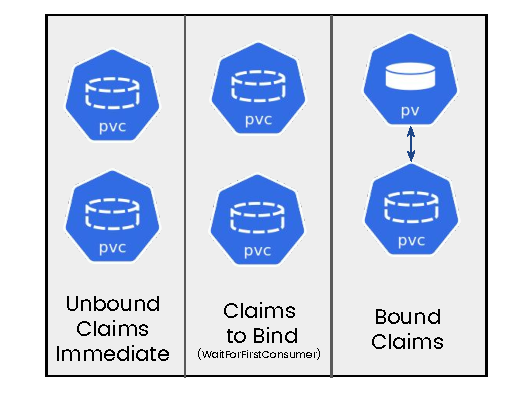
\includegraphics[width=0.6\textwidth]{resources/volumebinding-prefilter.pdf}
      \caption{VolumeBinding plugin's PreFilter method splits the PVCs a Pod references into 3 categories}
      \label{figure:volumebinding-prefilter}
\end{figure}

\subsection*{Filter phase}

The \co{VolumeBinding} plugin's \co{Filter()} method takes as input a Pod to be
scheduled, the bound and unbound claims the Pod references and a node. It checks
if the claims of the Pod are compatible with the node. In particular:

\begin{itemize}
      \tightlist
      \item For each \textit{bound claim}, it checks if the bound PV is
            accessible from the node, according to its node affinity. If a PV is
            not accessible, the Pod can not be scheduled on the examined node.
      \item For each \textit{claim to bind}, it checks if there is any unbound
            PV that matches the claim requests. If such a PV exists, it creates
            a binding for the claim with the PV in its cache. The remaining
            claims to bind, for which the plugin did not manage to find a
            matching PV, are claims that must be dynamically provisioned
            (hereafter referred to as \textit{``claims to provision''}).
      \item For each \textit{claim to provision}, it checks if the
            \co{StorageClass} the PVC requests supports dynamic provisioning and
            if there is enough storage capacity accessible from the node. If
            not, the Pod can not be scheduled on the node. At this step, the
            VolumeBinding plugin considers the storage capacity.
\end{itemize}

The current implementation of the scheduler checks if there is enough capacity
for each claim to dynamically provision by calling the \co{hasEnough()} method
with a single claim as input. It lists from the API Server all
\co{CSIStorageCapacity} objects and checks if any of them matches the
\co{StorageClass} of the PVC, is accessible from the examined node, and the
reported capacity on the object is greater than the requested capacity of the
PVC. If such a CSIStorageCapacity exists, the node has enough space for the
given claim to be dynamically provisioned.


For the sake of completeness, we expose the algorithm of the \co{Filter()}
method in Algorithm~\ref{alg:vol-binding-filter}.

\subsection*{PreBind phase}

As we explained, the VolumeBinding plugin's \co{Filter} phase tries to find PVs
for the unbound PVCs of the Pod; otherwise, it tries to dynamically provision
volumes for them.

During the \texttt{PreBind} phase, the VolumeBidning plugin executes the
following actions:
\begin{enumerate}
      \item For each PVC it found a matching PV, writes to the API Server the
            binding, i.e., it updates the PV to point to the PVC.
      \item For each PVC that needs provisioning, it updates the PVC on the API
            Server with the ``selected node annotation'' \footnote{The selected
                  node annotation: \co{volume.kubernetes.io/selected-node}} to signal
            the external provisioner that a volume for the PVC must be
            dynamically provisioned on a topology segment that is accessible
            from the selected node.
      \item  It then polls the API Server till all the unbound PVCs become fully
            bound. If the selected node annotation of any claim that needs
            provisioning is removed, the \co{PreBind} phase fails, and the
            scheduler cancels the current scheduling attempt.
      \item The scheduler will retry scheduling the Pod later.
\end{enumerate}


We shall point out that removing the selected node annotation from a dynamically
provisioned claim is a mechanism for the external provisioner to signal back to
the scheduler that the volume provisioning failed, and the scheduler shall retry
scheduling the Pod.




Here is an example of how the mechanism of the selected node  removal proves
useful:
\begin{enumerate}
      \tightlist
      \item The reported storage capacity information on the node is outdated:
            it indicates a reasonable quantity of storage, but the actual
            capacity is zero.
      \item The scheduler decides to schedule the Pod on that node based on the
            outdated capacity report.
      \item The scheduler decides to provision the PVC on the node and sets the
            selected node annotation.
      \item The external provisioner tries to provision the volume but fails
            since the available storage capacity is zero. It responds to the
            external provisioner with a \co{ResourceExhausted} status code.
      \item The external provisioner handles the \co{ResourceExhausted} status
            code and removes the selected node annotation from the PVC.
      \item The VolumeBinding plugin fails, and the scheduler cancels the
            scheduling attempt.
      \item The scheduler retries later, taking into consideration the possibly
            updated storage capacity information.
\end{enumerate}


For the sake of completeness, we expose the algorithm of the \co{PreBind()}
method in Algorithm~\ref{alg:vol-binding-prebind}.

\subsection{Shortcomings \& Proposed Extensions}

According to the previous analysis of the algorithms, the current design of the
Scheduler has the following limitations:
\begin{enumerate}
      \item The VolumeBinding plugin's Filter method uses the
            \co{CSIStorageCapacity} objects to fetch information for the
            available storage capacity. This API object was introduced as an
            alpha feature in Kubernetes 1.19 and became beta on Kubernetes
            version 1.21. The major cloud providers follow the policy not to
            enable alpha features on their services. As a result, the
            \co{CSIStorageCapacity} object is not available on clusters that run
            Kubernetes versions earlier than 1.21 on most cloud providers. That
            is a significant problem since many enterprises do not run the
            latest Kubernetes versions for stability reasons. In our case, our
            clients are running Kubernetes 1.19 and 1.20 clusters and, despite
            that, need to schedule Pods with local storage consideration.
      \item The current design rationale of the VolumeBinding plugin's method
            does not consider the total capacity required for provisioning
            multiple PVCs of a single Pod. Instead, it checks if there is enough
            capacity for each PVC separately. That is a crucial problem: if a
            Pod references multiple unbound PVCs and there is not enough space
            for all of them, some of them will get provisioned, and the rest
            will fail. Then all future scheduling decisions will be limited by
            the already provisioned volumes, and the Pod will be stuck.
            Considering the total storage required for all the PVCs would
            minimize the possibility of bumping onto the previous problem (yet,
            some race conditions may cause this).
\end{enumerate}

Since the upstream design comes with the aforementioned limitations, we propose
extending the Kubernetes Scheduler and deploying our extended scheduler on the
clusters. The proposed design consists of the following parts:
\begin{itemize}
      \tightlist
      \item Extend the Rok CSI Node component to report the available capacity
            of each node.
      \item Extend the Rok CSI Controller component to respond with an
            \co{ResourceExhausted} error status code to the \co{CreateVolume}
            request when the provisioning of a volume fails due to insufficient
            storage.
      \item Extend the Kubernetes Scheduler's VolumeBinding plugin to consider
            the total storage required by multiple PVCs and compare it against
            the reported free capacity of each node.
      \item Deploy the extended scheduler on the cluster.
      \item Deploy a webhook to mutate Pods to be scheduled by our custom
            scheduler.
\end{itemize}

We analyze each part of the design in the following paragraphs.

\subsubsection{Extend Rok CSI Node}
\label{section:capacity-annotation}
The \co{CSIStorageCapacity} objects for the capacity report can not be
back-ported to previous Kubernetes versions; moreover, adding a similar object
using a Custom Resource would be too much of a hassle. For these reasons, we
decide to report the capacity of each node as an annotation on the corresponding
\co{Node} object. We use the \co{rok.arrikto.com/capacity} key for the
annotation. Hereafter we refer to it as the ``\textit{capacity annotation}''.

The Rok CSI Node on each cluster node calculates the available storage and
updates the capacity annotation. It issues commands to the Logical Volume
Manager (LVM) of the node to fetch the free space of the Rok Volume Group and
updates the \co{Node} object on the API Server.

An illustration of the mechanism is shown in Figure \ref{fig:csi-capacity}.

\begin{figure}[ht]
      \centering
      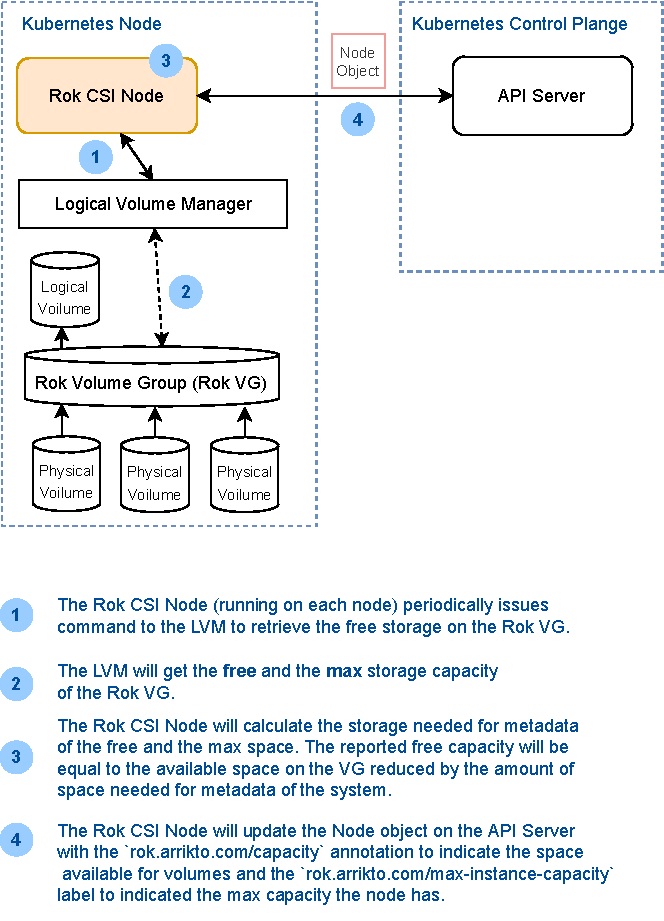
\includegraphics[width=0.9\textwidth]{resources/csi-storage-calculation.pdf}
      \caption{Rok CSI Node's capacity report mechanism}
      \label{fig:csi-capacity}
\end{figure}


\subsubsection{Extend Rok CSI Controller}
We extend the Rok CSI Controller to return the \co{GRPCResourceExhausted} status
code in response to the \co{CreateVolume} call of the external provisioner when
the creation of a volume fails due to insufficient storage capacity.

\subsubsection{Extend the VolumeBinding Plugin}
\label{section:volume-plugin-extensions}

We propose the extension of the \co{VolumeBidning} plugin's \co{Filter} phase as
follows:
\begin{enumerate}
      \tightlist
      \item When checking the PVCs of the Pod that need provisioning
            (\co{checkVolumeProvisions()} method), select all the Rok PVCs
            \footnote{PVCs provisioned by the \co{rok.arrikto.com}
                  provisioner.} (hereafter referred to as the ``\textit{Rok
                  claims to provision}'') and check if there is enough capacity
            for the total storage they request.
      \item Check if there is enough capacity for the Rok claims to dynamically
            provision, as follows:
            \begin{enumerate}
                  \tightlist
                  \item Calculate the total capacity requested for Rok claims
                        that need dynamic provisioning by summing their
                        requests.
                  \item Check if the examined node has the Rok capacity
                        \footnote{The Rok capacity annotation:
                              \texttt{rok.arrikto.com/capacity}} annotation.
                  \item If the annotation \textit{does not exist}, or if it
                        exists but is not a valid integer number, the Rok claims
                        can not be provisioned on the node. The absence of the
                        annotation indicates that the Rok CSI driver is not
                        running on the node; consequently, the claims can not be
                        provisioned there.
                  \item If the annotation \textit{exists}, check if the reported
                        available capacity is greater or equal to the total
                        capacity the Rok claims request. If the condition holds,
                        there is enough capacity, and the Rok claims of the Pod
                        can be provisioned on the node. Otherwise, there is
                        insufficient capacity; the Rok claims can not be
                        provisioned, and the Pod can not be scheduled on the
                        node.
            \end{enumerate}
      \item Maintain backward compatibility by not modifying the handling of
            non-Rok PVCs, which may not be local. Our design splits the PVCs
            into local Rok PVCs and non-Rok PVCs; it only extends how the
            scheduler handles the Rok PVCs. PVCs provisioned by other storage
            providers will not be affected by our changes.
\end{enumerate}


\subsubsection{Deploy the Custom Rok Scheduler}

The \co{kube-cheduler} runs by default on each cloud provider as part of the
Kubernetes control plane and is the default scheduler used for scheduling Pods.
The cloud providers hide the control plane from the end-user of their services,
so there is no option to replace the instance of the running scheduler.

Due to this limitation, we deploy our scheduler on the cluster that runs the
extended VolumeBinding plugin. Hereafter we refer to our custom scheduler as the
``Rok Scheduler''.


\subsubsection{Deploy the Rok Scheduler Webhook}

Since we deploy the Rok Scheduler without replacing the default Kubernetes
Scheduler of the cluster, each Pod shall specify which scheduler shall schedule
it by setting its \co{spec.schedulerName} field. If the field is not set, the
default scheduler is used.

We do not want each user to manually set the name of the scheduler on the Pod;
this would allow users to bypass the scheduling policy we set, is prone to
errors, and is a tedious process. We need an automatic way to achieve this. The
solution for automating the task is a mutating webhook.

We deploy a mutating webhook on the cluster, hereafter referred to as the ``Rok
Scheduler webhook'', which admits newly created Pods in specific namespaces of
the cluster and adds the name of the Rok Scheduler on the Pod's spec. The
proposed design is illustrated in Figure \ref{fig:rok-scheduler-webhook}.


\begin{figure}[ht]
      \centering
      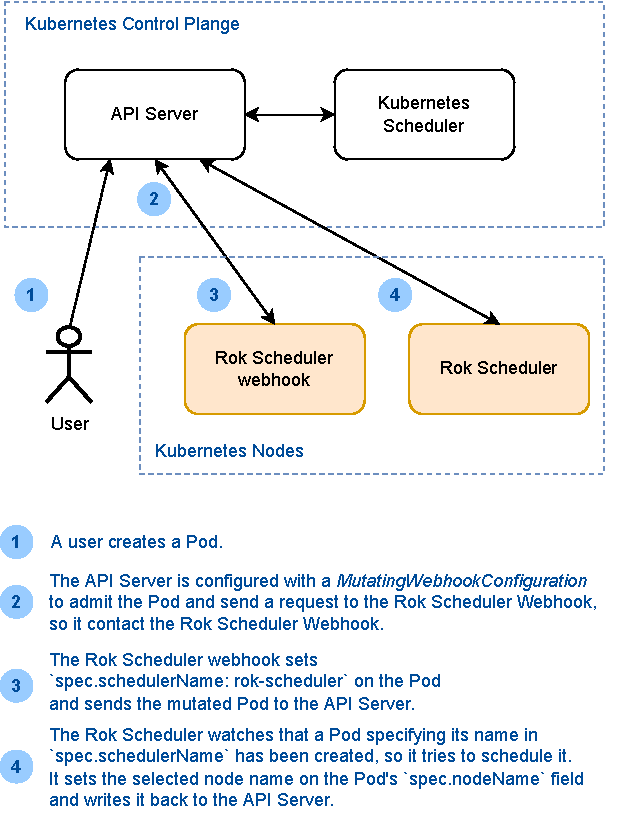
\includegraphics[width=0.9\textwidth]{resources/webhook-design.pdf}
      \caption{Deployment of Rok Scheduler along with its webhook}
      \label{fig:rok-scheduler-webhook}
\end{figure}


\subsubsection{End-to-End Story of the Proposed Design}

With the new design, this is the succession of interactions that will take place
between the various components:

\begin{enumerate}
      \tightlist
      \item A user creates a Pod that references unbound Rok PVCs.
      \item The Kubernetes MutatingAdmissionWebhook admission controller sends a
            request to the Rok Scheduler webhook to mutate the Pod.
      \item The Rok Scheduler webhook adds the name of the Rok Scheduler on the
            spec of the Pod and responds to the API Server with the mutated Pod.
      \item The Rok Scheduler sees the Pod's spec specifies \co{scedhulerName:
                  rok-scheduler} and handles its scheduling.
      \item The VolumeBinding plugin \co{Filter} method of the Rok Scheduler
            calculates the total capacity requested by the unbound Rok PVCs. It
            compares it against the value of the capacity annotation of the node
            it examines. It considers feasible nodes only these with enough
            capacity for the total requested storage.
      \item The Rok Scheduler selects a node to place the Pod and adds the
            selected node annotation on the PVCs of the Pod to be provisioned.
      \item The external provisioner of the Rok CSI sees the selected node
            annotation on the unbound Rok PVC and submits a \co{CreateVolume}
            GRPC call to the Rok CSI Controller component to provision a volume
            accessible from the selected node.
      \item The Rok CSI Controller handles the request and submits a job for
            volume creation.
      \item The Rok CSI Node component on the selected node executes the job. To
            provision a logical volume, it issues a \co{lvcreate} command to the
            LVM.
      \item If there is not enough space on the Rok Volume Group, the
            \co{lvcreate} command will fail with \co{ResourceExhausted} status
            code, the job will fail, and the Rok CSI Node will report the reason
            and message of failure of the job to Rok.
      \item The Rok CSI Controller component sees that the job failed and parses
            the error message; it determines that it is due to insufficient
            storage capacity and responds with \co{ResourceExhausted} code
            status to the external provisioner's \co{CreateVolume} call.
      \item The external provisioner handles the \co{ResourceExhausted} error by
            removing the selected node annotation from the Rok PVC.
      \item The \co{PreBind} method of the VolumeBinding plugin of the Rok
            Scheduler notices that the selected node annotation was removed from
            the PVC and aborts the current scheduling attempt.
      \item The Rok Scheduler will attempt to scheduler the Pod again in the
            future.
\end{enumerate}
% TODO: Reorder algos?

\clearpage
\begin{algorithm}[h]
      \caption{The scheduler's VolumeBinding plugin: PreBind() method}
      \label{alg:vol-binding-prebind}
      \KwIn{\co{pod}: the Pod to be scheduled \\ \co{claimsToBind}: PVCs to bind
            \\ \co{claimsToProvision}: PVCs to provision \\ \co{node}: the
            selected node} \KwResult{Binds unbound PVCs of the Pod with PVs.}
      \begin{enumerate}[leftmargin=0.5cm]
            \tightlist
            \item Initiate the binding of \co{claimsToBind} by updating the API
                  Server with the binding of the PV to its matching PVC.
            \item Trigger the provisioning of \co{claimsToProvision} by updating
                  the API Server object of each PVC with the selected node
                  annotation.
            \item Wait for PVCs to be completely bound by the PV controller:
                  \begin{enumerate}[]
                        \tightlist
                        \item For each claim in \co{claimsToProvision}:
                              \begin{enumerate}
                                    \item Check its selected node annotation.
                                    \item \lIf{the annotation was
                                                removed}{cancel the scheduling attempt}
                              \end{enumerate}

                        \item For each claim in \co{claimsToProvision}, check if
                              the bidirectional binding of the claim to the
                              corresponding PV has completed.
                        \item \lIf{the operation times out}{return error}
                  \end{enumerate}
      \end{enumerate}
\end{algorithm}
\begin{algorithm}[H]
      \caption{The scheduler's VolumeBinding plugin: PreFilter() method}
      \label{alg:vol-binding-prefilter}
      \KwIn{\texttt{pod}: the Pod to be scheduled}
      \KwResult{Update the CycleState of the scheduler with the PVCs the Pod uses.}
      \begin{enumerate}[leftmargin=0.5cm]
            \tightlist
            \item \lIf {the Pod does not reference any PVCs}{return nil}
            \item Otherwise, split the PVCs into 3 categories:
                  \begin{enumerate}
                        \tightlist
                        \item \co{boundClaims}: PVCs bound with a PV.
                        \item \co{claimsToBind}: Unbound PVCs with \co{WaitForFirstConsumer}
                              (delayed) binding mode.
                        \item \co{unboundClaimsImmediate}: Unbound PVCs with \co{Immediate} binding mode.
                  \end{enumerate}
            \item \lIf{\co{unboundClaimsImmediate} is non-empty}{return error; abort the scheduling attempt}
            \item Store the \co{boundClaims} and \co{claimsToBind} in the \co{CycleState} of the scheduler.
                  \tightlist
      \end{enumerate}
\end{algorithm}
\clearpage
\begin{algorithm}[h]
      \caption{The scheduler's VolumeBinding plugin: Filter() method}
      \label{alg:vol-binding-filter}
      \KwIn{\texttt{pod}: the Pod to be scheduled
            \\ \texttt{claimsToBind}: PVCs of the Pod to bind
            \\ \texttt{boundClaims}: PVCs of the Pod that are bound
            \\ \co{node}: the \co{Node} to check against.}
      \KwResult{Checks if the PVCs of the Pod are compatible with the node}
      \begin{enumerate}[leftmargin=0.5cm]
            \tightlist
            \item Call \co{FindPodVolumes(pod, state.boundClaims, state.claimsToBind, node)}
                  to check if all of the Pod's PVCs can be satisfied by the node:
                  \begin{enumerate}
                        \item For each (bound) PVC in \co{boundClaims}:
                              \begin{enumerate}
                                    \tightlist
                                    \item Get the PV it is bound to.
                                    \item \lIf{the PV's node affinities do not match the node}{the node is not feasible for the Pod}
                              \end{enumerate}
                        \item For each (unbound) PVC in \co{claimsToBind}:
                              \begin{enumerate}
                                    \tightlist
                                    \item \lIf{the PVC has the selected node annotation and the selected node is not equal to the name of the examined Node}{return false (pod cannot be scheduled on the node.)}
                                    \item Try to find a matching PV for the PVC, to bind it to (by calling \co{findMatchingVolumes()}.
                                    \item \lIf{any matching PV was not found}{add the claim in list of volumes that must be provisioned (by calling \co{claimsToProvision()})}
                              \end{enumerate}
                  \end{enumerate}
            \item Call \co{checkVolumeProvisions(claimsToProvision)}, to check the claims that need provisioning:
                  \begin{enumerate}
                        \tightlist
                        \item For each claim in \co{claimsToProvision} :
                              \begin{enumerate}
                                    \tightlist
                                    \item Get the \co{StorageClass} that the PVC requests.
                                    \item \lIf{the \co{StorageClass} does not support dynamic provisioning}{return error}
                                    \item Check if there is enough capacity on the node, by calling \co{hasEnoughCapacity()}.
                                    \item \lIf{there is not enough capacity}{return error}
                              \end{enumerate}
                  \end{enumerate}
      \end{enumerate}
\end{algorithm}

\clearpage
\begin{algorithm}[h]
      \caption{The scheduler's VolumeBinding Plugin: hasEnough() method}
      \label{alg:vol-binding-has-enough}
      \KwIn{\texttt{claim}: the PVC to check
            \\ \co{node}: the \co{Node} to examine
      }
      \KwResult{Checks if there is enough capacity for PVC on the node.}
      \begin{enumerate}[leftmargin=0.5cm]
            \tightlist
            \item request \lar Storage size (in bytes) the PVC requests.
            \item Get the name of the provisioner from \co{StorageClass} the PVC requests.
            \item Get the \co{CSIDriver} object with the same name as the provisioner.
            \item \lIf{no such \co{CSIDriver} object exists}{return true (capacity tracking is not enabled)}
            \item \co{capacities} \lar List all the \co{CSIStorageCapacity} objects from the API Server.
            \item For each \co{capacity} in \co{capacities}:
                  \begin{enumerate}
                        \item \lIf{capacity.StorageClassName != storageClass.Name}{go to the next \co{capacity}}
                        \item \lIf{request $>$ capacity.Capacity}{go to next \co{capacity}}
                        \item Check if node has access to the specific topology, by checking the \co{capacity.NodeTopology} against the node's labels.
                        \item \lIf{node does not have access to the topology}{go to next \co{capacity}}
                        \item Return \co{true} (the node has access to enough capacity for the volume to be provisioned).
                  \end{enumerate}
            \item Return \co{false}, no CSIStorageCapacity with enough capacity for the PVC accessible from the node was found.
      \end{enumerate}
\end{algorithm}
\clearpage
